\documentclass[11pt,compress,t,notes=noshow, xcolor=table]{beamer}
\usepackage[]{graphicx}\usepackage[]{color}
% maxwidth is the original width if it is less than linewidth
% otherwise use linewidth (to make sure the graphics do not exceed the margin)
\makeatletter
\def\maxwidth{ %
  \ifdim\Gin@nat@width>\linewidth
    \linewidth
  \else
    \Gin@nat@width
  \fi
}
\makeatother

\definecolor{fgcolor}{rgb}{0.345, 0.345, 0.345}
\newcommand{\hlnum}[1]{\textcolor[rgb]{0.686,0.059,0.569}{#1}}%
\newcommand{\hlstr}[1]{\textcolor[rgb]{0.192,0.494,0.8}{#1}}%
\newcommand{\hlcom}[1]{\textcolor[rgb]{0.678,0.584,0.686}{\textit{#1}}}%
\newcommand{\hlopt}[1]{\textcolor[rgb]{0,0,0}{#1}}%
\newcommand{\hlstd}[1]{\textcolor[rgb]{0.345,0.345,0.345}{#1}}%
\newcommand{\hlkwa}[1]{\textcolor[rgb]{0.161,0.373,0.58}{\textbf{#1}}}%
\newcommand{\hlkwb}[1]{\textcolor[rgb]{0.69,0.353,0.396}{#1}}%
\newcommand{\hlkwc}[1]{\textcolor[rgb]{0.333,0.667,0.333}{#1}}%
\newcommand{\hlkwd}[1]{\textcolor[rgb]{0.737,0.353,0.396}{\textbf{#1}}}%
\let\hlipl\hlkwb

\usepackage{framed}
\makeatletter
\newenvironment{kframe}{%
 \def\at@end@of@kframe{}%
 \ifinner\ifhmode%
  \def\at@end@of@kframe{\end{minipage}}%
  \begin{minipage}{\columnwidth}%
 \fi\fi%
 \def\FrameCommand##1{\hskip\@totalleftmargin \hskip-\fboxsep
 \colorbox{shadecolor}{##1}\hskip-\fboxsep
     % There is no \\@totalrightmargin, so:
     \hskip-\linewidth \hskip-\@totalleftmargin \hskip\columnwidth}%
 \MakeFramed {\advance\hsize-\width
   \@totalleftmargin\z@ \linewidth\hsize
   \@setminipage}}%
 {\par\unskip\endMakeFramed%
 \at@end@of@kframe}
\makeatother

\definecolor{shadecolor}{rgb}{.97, .97, .97}
\definecolor{messagecolor}{rgb}{0, 0, 0}
\definecolor{warningcolor}{rgb}{1, 0, 1}
\definecolor{errorcolor}{rgb}{1, 0, 0}
\newenvironment{knitrout}{}{} % an empty environment to be redefined in TeX

\usepackage{alltt}
\newcommand{\SweaveOpts}[1]{}  % do not interfere with LaTeX
\newcommand{\SweaveInput}[1]{} % because they are not real TeX commands
\newcommand{\Sexpr}[1]{}       % will only be parsed by R
\newcommand{\xmark}{\ding{55}}%


\usepackage[english]{babel}
\usepackage[utf8]{inputenc}

\usepackage{dsfont}
\usepackage{verbatim}
\usepackage{amsmath}
\usepackage{amsfonts}
\usepackage{amssymb}
\usepackage{bm}
\usepackage{csquotes}
\usepackage{multirow}
\usepackage{longtable}
\usepackage{booktabs}
\usepackage{enumerate}
\usepackage[absolute,overlay]{textpos}
\usepackage{psfrag}
\usepackage{algorithm}
\usepackage{algpseudocode}
\usepackage{eqnarray}
\usepackage{arydshln}
\usepackage{tabularx}
\usepackage{placeins}
\usepackage{tikz}
\usepackage{setspace}
\usepackage{colortbl}
\usepackage{mathtools}
\usepackage{wrapfig}
\usepackage{bm}
\usepackage{amsmath}
\usepackage{pifont}

\usetikzlibrary{shapes,arrows,automata,positioning,calc,chains,trees, shadows}
\tikzset{
  %Define standard arrow tip
  >=stealth',
  %Define style for boxes
  punkt/.style={
    rectangle,
    rounded corners,
    draw=black, very thick,
    text width=6.5em,
    minimum height=2em,
    text centered},
  % Define arrow style
  pil/.style={
    ->,
    thick,
    shorten <=2pt,
    shorten >=2pt,}
}

\usepackage{subfig}

% Defines macros and environments
\usepackage{../../style/lmu-lecture}


\let\code=\texttt
\let\proglang=\textsf

\setkeys{Gin}{width=0.9\textwidth}

\setbeamertemplate{frametitle}{\expandafter\uppercase\expandafter\insertframetitle}

\usepackage{bbm}
% basic latex stuff
\newcommand{\pkg}[1]{{\fontseries{b}\selectfont #1}} %fontstyle for R packages
\newcommand{\lz}{\vspace{0.5cm}} %vertical space
\newcommand{\dlz}{\vspace{1cm}} %double vertical space
\newcommand{\oneliner}[1] % Oneliner for important statements
{\begin{block}{}\begin{center}\begin{Large}#1\end{Large}\end{center}\end{block}}


%new environments
\newenvironment{vbframe}  %frame with breaks and verbatim
{
 \begin{frame}[containsverbatim,allowframebreaks]
}
{
\end{frame}
}

\newenvironment{vframe}  %frame with verbatim without breaks (to avoid numbering one slided frames)
{
 \begin{frame}[containsverbatim]
}
{
\end{frame}
}

\newenvironment{blocki}[1]   % itemize block
{
 \begin{block}{#1}\begin{itemize}
}
{
\end{itemize}\end{block}
}

\newenvironment{fragileframe}[2]{  %fragile frame with framebreaks
\begin{frame}[allowframebreaks, fragile, environment = fragileframe]
\frametitle{#1}
#2}
{\end{frame}}


\newcommand{\myframe}[2]{  %short for frame with framebreaks
\begin{frame}[allowframebreaks]
\frametitle{#1}
#2
\end{frame}}

\newcommand{\remark}[1]{
  \textbf{Remark:} #1
}


\newenvironment{deleteframe}
{
\begingroup
\usebackgroundtemplate{
\includegraphics[width=\paperwidth,height=\paperheight]{../style/color/red.png}}
 \begin{frame}
}
{
\end{frame}
\endgroup
}
\newenvironment{simplifyframe}
{
\begingroup
\usebackgroundtemplate{
\includegraphics[width=\paperwidth,height=\paperheight]{../style/color/yellow.png}}
 \begin{frame}
}
{
\end{frame}
\endgroup
}\newenvironment{draftframe}
{
\begingroup
\usebackgroundtemplate{
\includegraphics[width=\paperwidth,height=\paperheight]{../style/color/green.jpg}}
 \begin{frame}
}
{
\end{frame}
\endgroup
}
% https://tex.stackexchange.com/a/261480: textcolor that works in mathmode
\makeatletter
\renewcommand*{\@textcolor}[3]{%
  \protect\leavevmode
  \begingroup
    \color#1{#2}#3%
  \endgroup
}
\makeatother





\input{../../latex-math/basic-math.tex}
\input{../../latex-math/basic-ml.tex}

\newcommand{\titlefigure}{figure_man/the_inducer_web.png}
\newcommand{\learninggoals}{
\item Understand that a supervised learner fits models automatically from training data
% \item Understand that a learner is an algorithm or function for a certain
    % hypothesis space, which receives training data and outputs
    % the optimal model / parametrization from that function space for that data
}

\title{Introduction to Machine Learning}
% \author{Bernd Bischl, Christoph Molnar, Daniel Schalk, Fabian Scheipl}
\institute{\href{https://compstat-lmu.github.io/lecture_i2ml/}{compstat-lmu.github.io/lecture\_i2ml}}
\date{}

\begin{document}

\lecturechapter{ML-Basics: Learner}
\lecture{Introduction to Machine Learning}


\begin{vbframe}{Supervised Learning Example}

Imagine we want to investigate how working conditions affect productivity of employees.

\begin{itemize}
	\item It is a \textbf{regression} task since the target \emph{productivity} is continuous.
	% \item It is \textbf{learn to explain} if we want to tweak the features in the future to increase productivity and \textbf{learn to predict} if we need a forecast.
	\item We collect data about worked minutes
per week (\emph{productivity}), how many people work in the same office as the
employee in question, and the employee's salary.
\end{itemize}

% FIGURE SOURCE: https://docs.google.com/presentation/d/1qIWHJq-iZqfUsLLJD81Z9LhobGTIN3sDHTevnm5dxZ0/edit?usp=sharing
\begin{center}
  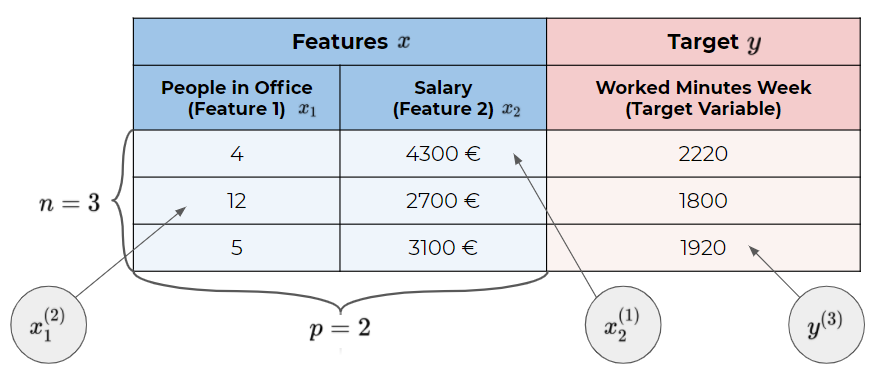
\includegraphics[width = 0.7\textwidth]{figure_man/data_table}
\end{center}

\framebreak

How could we construct a model from these data?\\[1ex]

We could investigate the data manually and come up with a simple, hand-crafted rule such as:

	\begin{itemize}
		\item The baseline productivity of an employee with salary 3000 and 7 people in the office is 1850 minutes
		\item A decrease of 1 person in the office increases productivity by 30
		\item An increase of the salary by 100 increases productivity by 10
	\end{itemize}

=> Obviously, this is neither feasible nor leads to a good model
\end{vbframe}



\begin{vbframe}{Idea of Supervised Learning}


\textbf{Goal:} Automatically identify the fundamental functional relation in the data
  that maps an object's features to the target.

\begin{itemize}

  \item \textbf{Supervised} learning means we make use of \emph{labeled}
  data for which we observed the outcome.

  % \item For new data we can only observe the features but not the target.

  \item We use the labeled data to learn a model f.

  \item Ultimately, we use our model to compute predictions for
  \textbf{new} data whose target values are unknown.

\end{itemize}

\begin{center}
% FIGURE SOURCE: https://docs.google.com/presentation/d/1WLPubv9vxLL-JIlHAtsvTBBG5pbF4xgRGW_prkOAEnE/edit?usp=sharing Page 4
  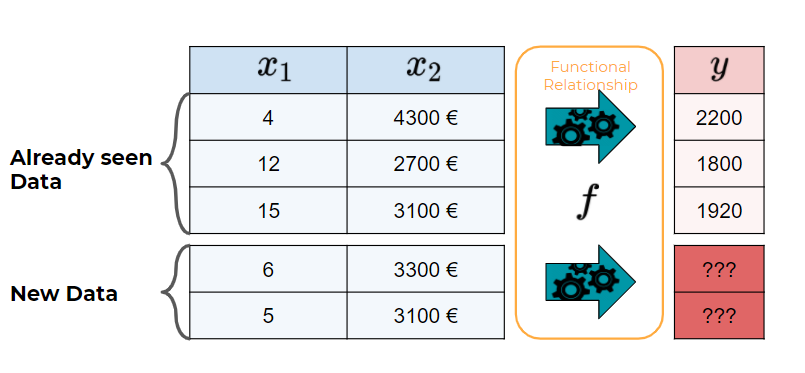
\includegraphics[width=0.7\textwidth]{figure_man/what_is_a_model_web}
\end{center}
\end{vbframe}

\framebreak

% \begin{vbframe}{Idea of Supervised Learning}

% \begin{itemize}


  % \item However, in practical applications we don't and must try to
  % \textbf{learn} it from give examples.

%  $\rightarrow$ We call such an assumed mapping a \textbf{model} $f$.

  % \item In machine learning, we rely on computers, which is why the model
  % itself, as well as all feature and target values, need to be
  % \textbf{computable}.

% \end{itemize}

%\framebreak

%\begin{itemize}

%  % \item The set-up in supervised learning will typically look like this:
%  %
%  % \begin{itemize}
%  %
%  %   \item We restrict our options to a certain class of functions,
%  %
%  %   \item choose some metric to evaluate model candidates,
%  %
%  %   \item and try to find the best candidate in an efficient way.
%  %
%  % \end{itemize}
%  %
%  % \item This procedure is carried out by an algorithm called \textbf{learner} or
%  % \textbf{inducer}.


  % We can see that for objects with certain
  % patterns or properties, some values of the target are more likely than others.


  % \item Using the learned model, we can make \textbf{predictions} of the target, based on
  % the features of our data.

  % \item Knowing the \enquote{truth} allows us to test how well we have grasped
  % the nature of the underlying mapping: we just need to compare our predictions
  % to the actually observed values.

%  \framebreak

% \end{itemize}

% \end{vbframe}



% ------------------------------------------------------------------------------


\begin{vbframe}{Learner Definition}

\begin{itemize}

  \item The algorithm for finding our $f$ is called \textbf{learner}.
      It is also called \textbf{learning algorithm} or \textbf{inducer}.

  \item We prescribe a certain hypothesis space,
  the learner is our means of picking the best element from that space
  for our data set.

\item Formally, it maps training data $\D \in \allDatasets$ (plus a vector of \textbf{hyperparameter} control settings $\bm{\lambda} \in \bm{\Lambda}$) to a model:
\[\inducer: \preimageInducerShort \rightarrow \Hspace\]
% We can also adapt this concept to finding $\thetabh$ for parametric
% models:
% \[\inducer: \D \times \Lambda \rightarrow \Theta\]

\end{itemize}

  \begin{center}
    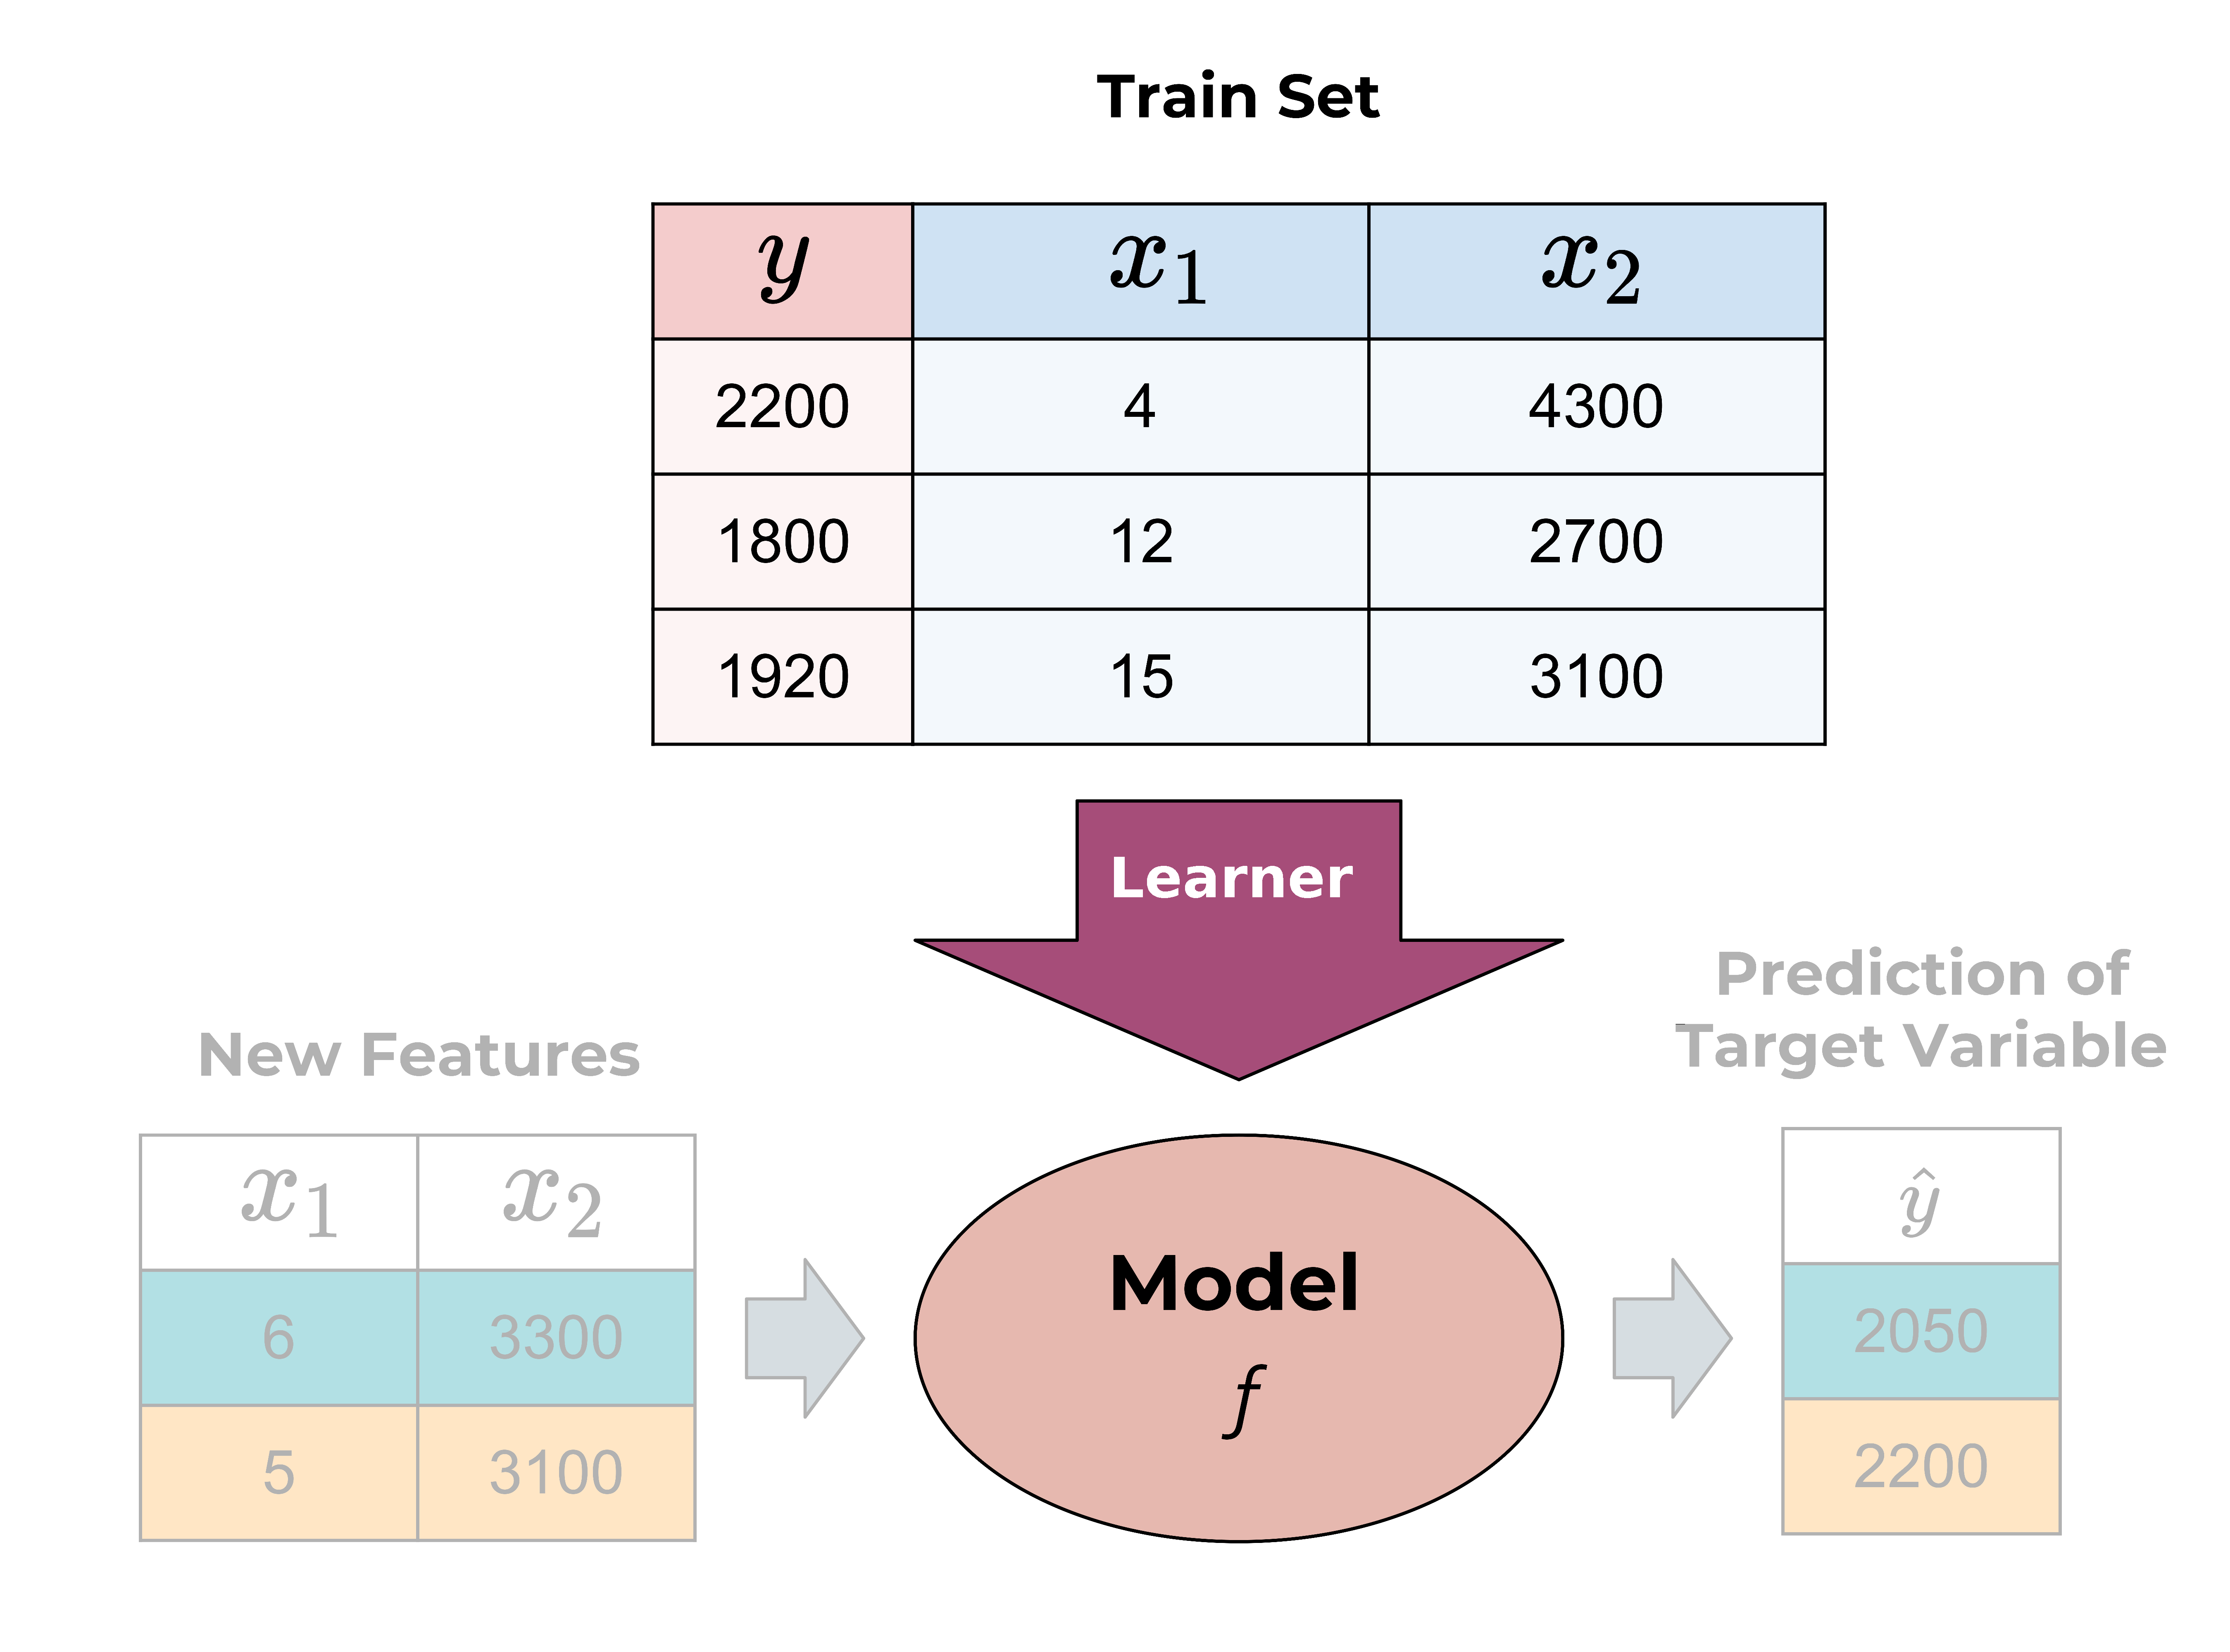
\includegraphics[width = 0.45\textwidth]{figure_man/the_inducer_web.png}
  \end{center}

\framebreak

As pseudo-code template it would work like this:
\begin{itemize}
  \item Learner has a defined model space of parametrized functions $\Hspace$.
  \item User passes data set $\Dtrain$ and control settings $\bm{\lambda}$.
  \item Learner sets parameters so that model
    matches data best.
  \item Optimal parameters $\thetabh$ or function $\fh$ is returned for later usage.

\end{itemize}

  \begin{center}
    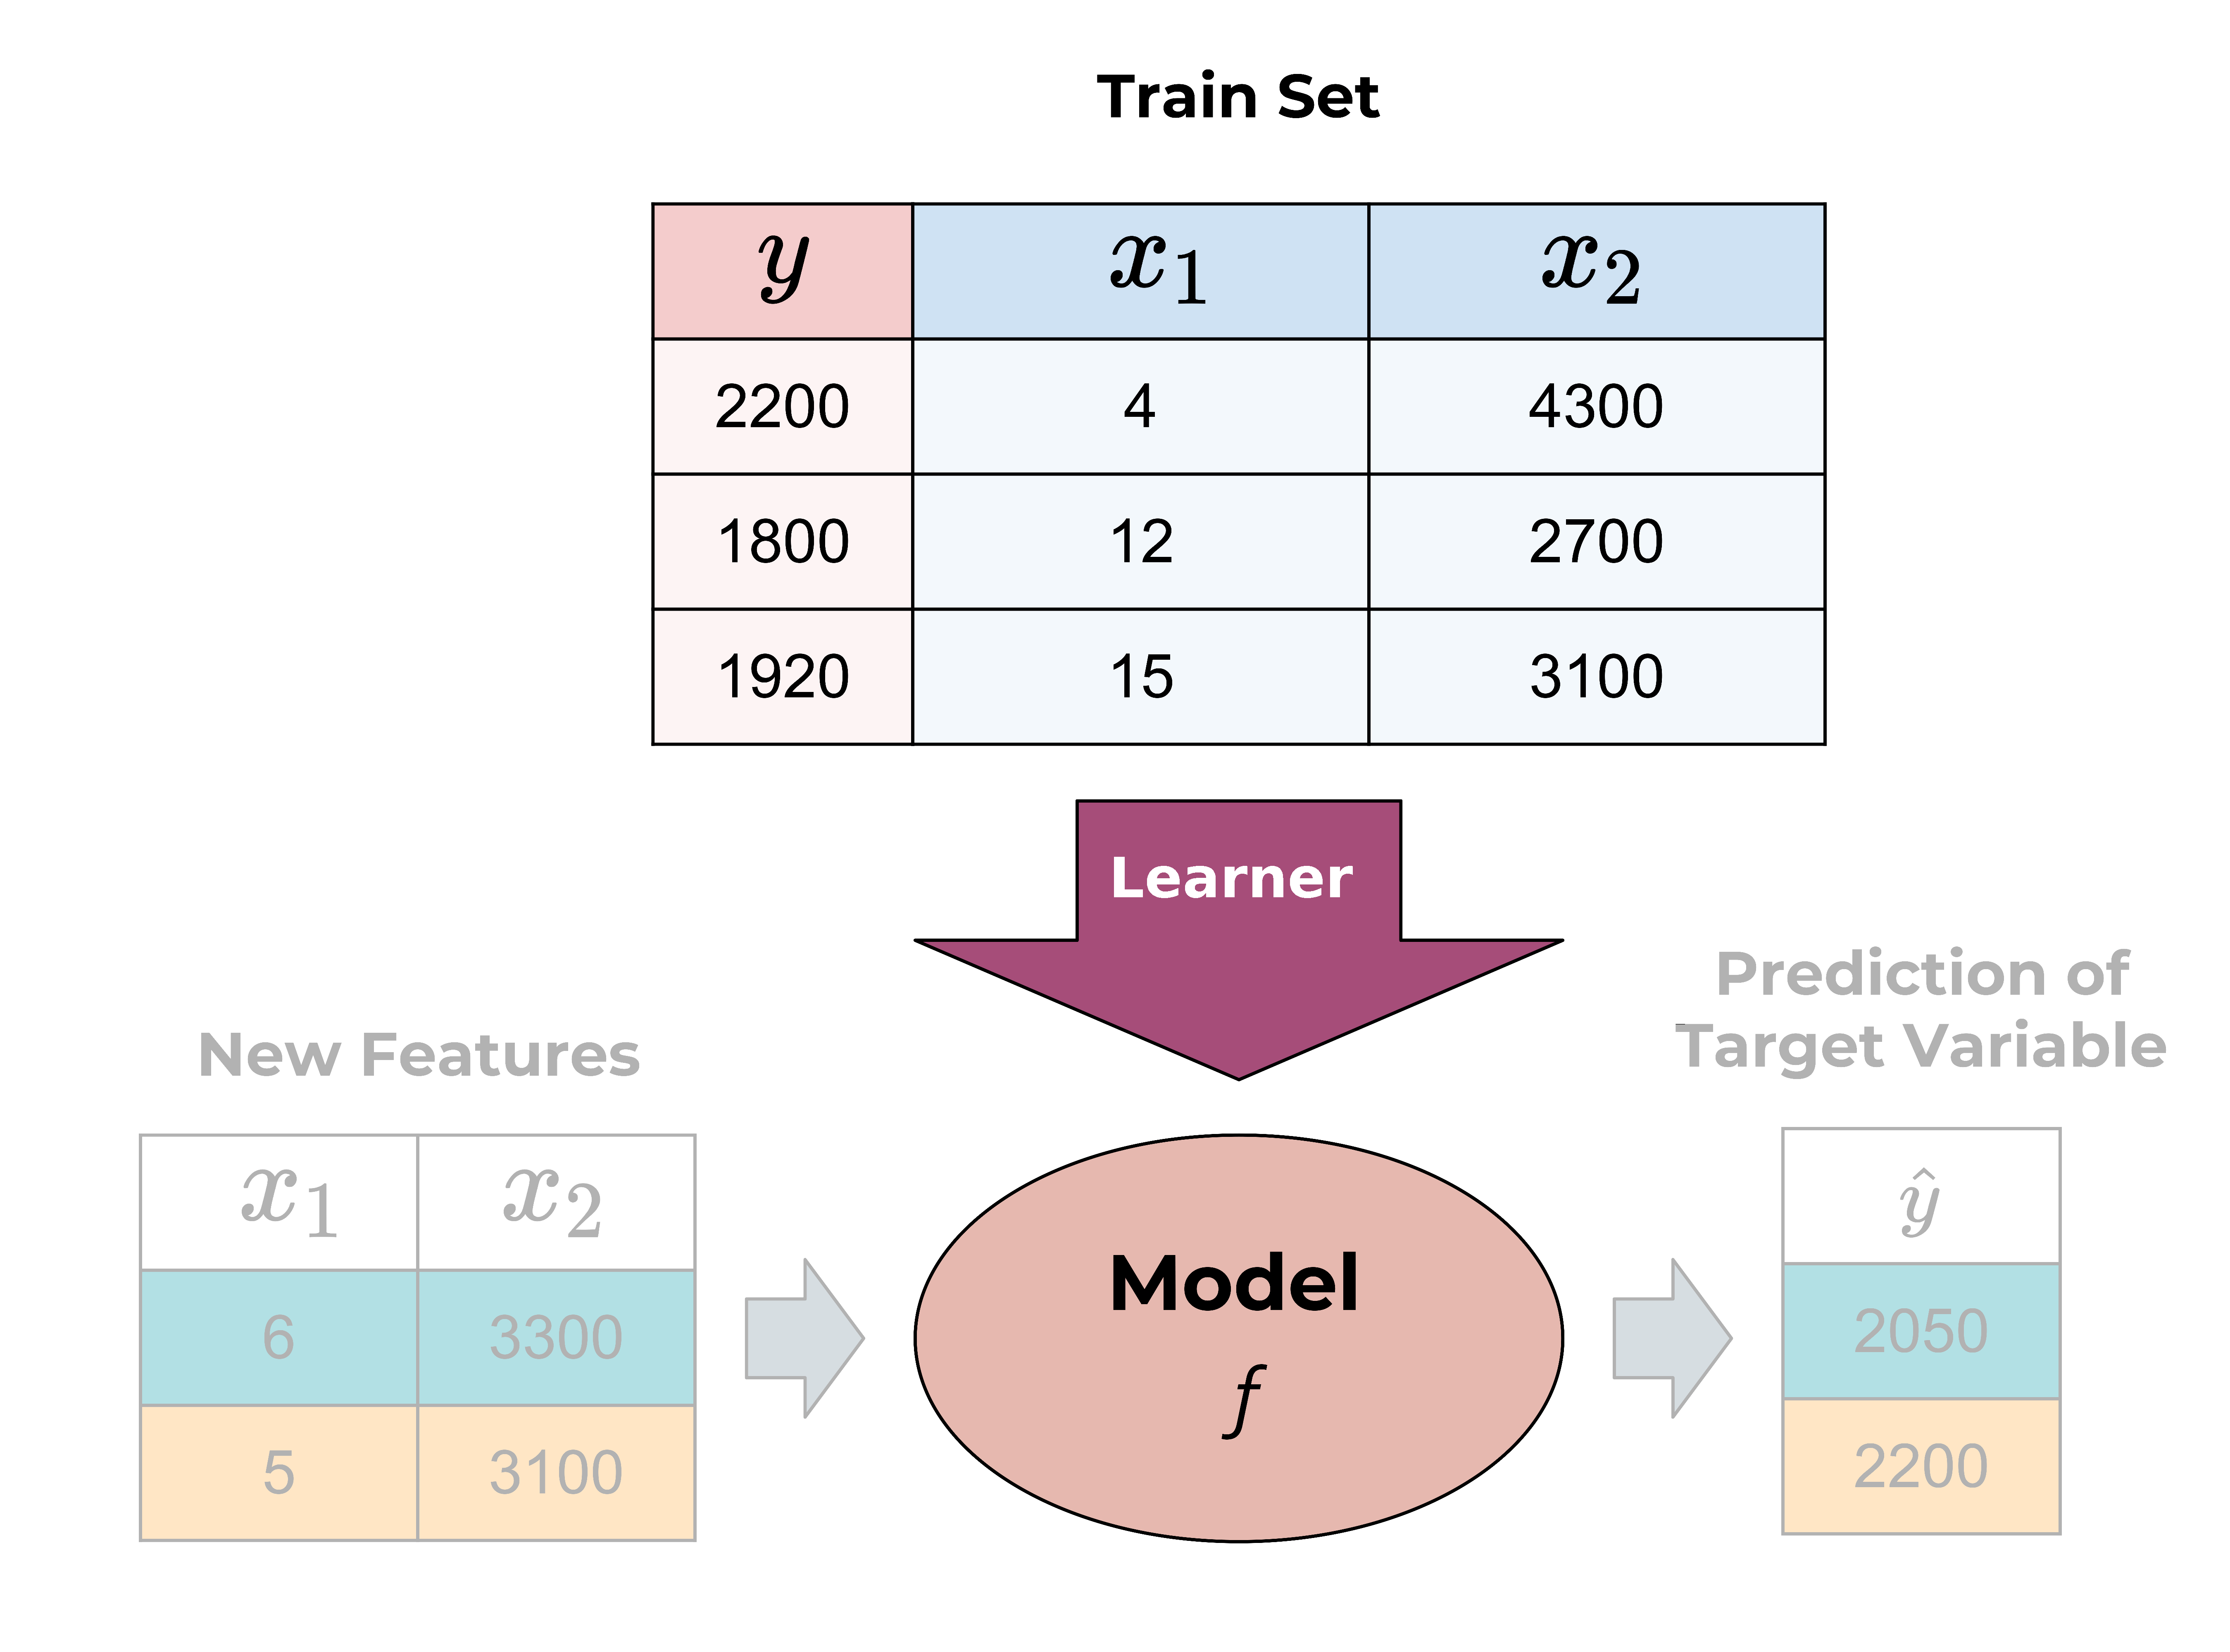
\includegraphics[width = 0.45\textwidth]{figure_man/the_inducer_web.png}
  \end{center}


\end{vbframe}






% ------------------------------------------------------------------------------

% \begin{vbframe}{Summary}
%
% \medskip
%
% \textbf{Supervised machine learning} is concerned with learning a function
% that predicts a certain \textbf{target} from an object's \textbf{features}
% from a set of examples for which both the features and the target are known.\\
% The function to be learned is restricted to come from a certain class of
% functions and its precise shape is defined in terms of a set of
% \textbf{parameters}.
%
% \end{vbframe}

% ------------------------------------------------------------------------------

\endlecture
\end{document}
